\documentclass[11pt]{article}

\usepackage[margin=0.82in]{geometry}
\usepackage{amsmath,amssymb,mathtools}
\usepackage{booktabs,tabularx,array}
\usepackage{microtype}
\usepackage{enumitem}
\usepackage{xcolor}
\usepackage{tikz}
\usetikzlibrary{arrows.meta,positioning,calc,fit,backgrounds,shapes.geometric}
\usepackage{xurl}
\usepackage[hidelinks]{hyperref}
\usepackage{fancyhdr}

\definecolor{ink}{RGB}{28,39,49}
\definecolor{navy}{RGB}{39,70,105}
\definecolor{teal}{RGB}{0,122,112}
\definecolor{gold}{RGB}{196,132,32}
\definecolor{coral}{RGB}{190,76,67}
\definecolor{plum}{RGB}{112,77,125}
\definecolor{mist}{RGB}{239,244,246}
\definecolor{paleteal}{RGB}{229,244,241}
\definecolor{palegold}{RGB}{250,242,224}
\definecolor{palecoral}{RGB}{250,233,231}
\definecolor{linegray}{RGB}{176,188,196}

\hypersetup{colorlinks=true,linkcolor=navy,citecolor=teal,urlcolor=navy}
\color{ink}
\setlength{\parindent}{0pt}
\setlength{\parskip}{0.56em}
\interfootnotelinepenalty=10000
\setlist{itemsep=0.25em,topsep=0.35em}
\renewcommand{\arraystretch}{1.18}

\pagestyle{fancy}
\fancyhf{}
\fancyhead[L]{\small\textcolor{navy}{REALITY IN NULL STEPS}}
\fancyhead[R]{\small\textcolor{ink!65}{Null-Edge Formalization Project}}
\fancyfoot[C]{\thepage}
\renewcommand{\headrulewidth}{0.3pt}

\newcommand{\ii}{\mathrm{i}}
\newcommand{\tr}{\operatorname{tr}}
\newcommand{\rank}{\operatorname{rank}}
\newcommand{\C}{\mathbb{C}}
\newcommand{\R}{\mathbb{R}}
\newcommand{\Mlabel}{\textcolor{teal}{\textsc{checked finite result}}}
\newcommand{\Tlabel}{\textcolor{navy}{\textsc{established physics}}}
\newcommand{\Clabel}{\textcolor{gold!80!black}{\textsc{open interpretation}}}

\newcommand{\widebox}[3]{%
  \begin{center}
  \fcolorbox{#1}{#2}{%
    \begin{minipage}{0.91\linewidth}
    \vspace{0.35em}\textbf{#3}\vspace{0.35em}
    \end{minipage}}
  \end{center}}

\newcommand{\claimbox}[2]{%
  \begin{center}
  \fcolorbox{teal}{paleteal}{%
    \begin{minipage}{0.91\linewidth}
    \textbf{#1}\quad #2
    \end{minipage}}
  \end{center}}

\tikzset{
  nullray/.style={very thick,teal,-{Latex[length=2.2mm]}},
  drift/.style={very thick,coral,-{Latex[length=2.2mm]}},
  transport/.style={thick,navy,-{Latex[length=2mm]}},
  faint/.style={thin,linegray},
  label/.style={font=\small,align=center,text=ink},
  channel/.style={draw=ink!45,fill=mist,rounded corners=2pt,
    minimum width=3.15cm,minimum height=1.45cm,align=center},
  dot/.style={circle,fill=ink,inner sep=1.7pt}
}

\begin{document}

\begin{titlepage}
\thispagestyle{empty}
\begin{center}
\vspace*{0.55in}
{\fontsize{31}{35}\selectfont\bfseries\textcolor{navy}{Reality in Null Steps}}\\[0.25em]
{\Large A visual guide to mass, motion, and geometry on a finite causal grid}\\[0.75em]
{\large Null-Edge Formalization Project}\\[0.2em]
{\textcolor{ink!65}{General-audience companion manuscript, July 9, 2026}}

\vspace{0.7in}
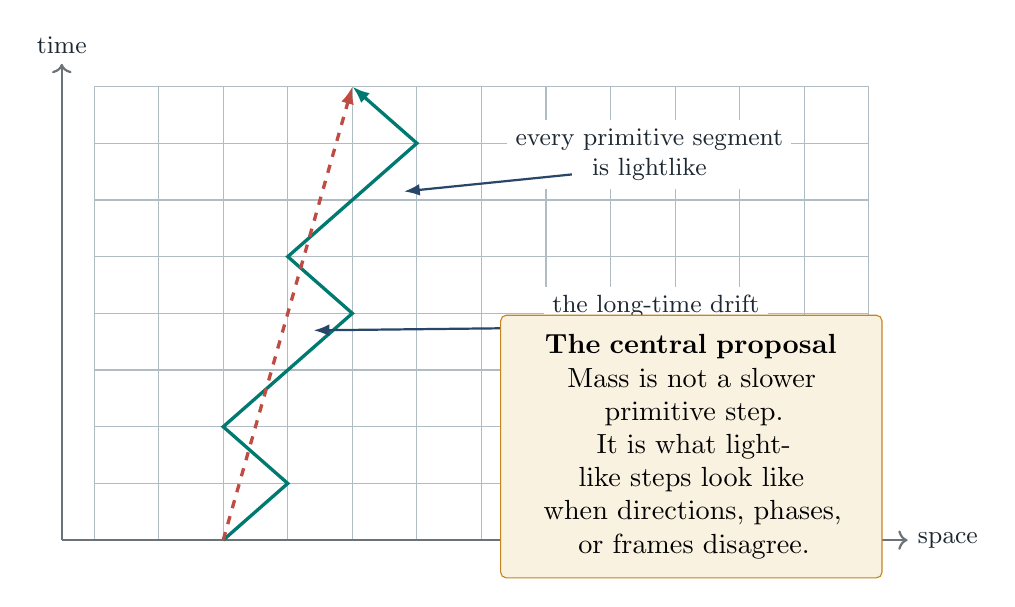
\begin{tikzpicture}[x=0.82cm,y=0.72cm]
  \foreach \x in {-6,-5,...,6} {\draw[faint] (\x,0)--(\x,8);}
  \foreach \y in {0,1,...,8} {\draw[faint] (-6,\y)--(6,\y);}
  \draw[->,thick,ink!65] (-6.5,0)--(-6.5,8.4) node[above,label]{time};
  \draw[->,thick,ink!65] (-6.5,0)--(6.6,0) node[right,label]{space};
  \draw[nullray] (-4,0)--(-3,1)--(-4,2)--(-3,3)--(-2,4)--(-3,5)--(-2,6)--(-1,7)--(-2,8);
  \draw[drift,dashed] (-4,0)--(-2,8);
  \node[label,fill=white,inner sep=3pt] at (2.6,6.8)
    {every primitive segment\\is lightlike};
  \draw[transport] (1.4,6.45)--(-1.2,6.15);
  \node[label,fill=white,inner sep=3pt] at (2.7,3.9)
    {the long-time drift\\is timelike};
  \draw[transport] (1.4,3.75)--(-2.6,3.7);
  \node[draw=gold,fill=palegold,rounded corners=2pt,align=center,
    text width=4.35cm,inner sep=7pt] at (3.25,1.65)
    {\textbf{The central proposal}\\Mass is not a slower primitive step.\\
     It is what lightlike steps look like\\when directions, phases, or frames disagree.};
\end{tikzpicture}

\vfill
\fcolorbox{navy}{mist}{\begin{minipage}{0.88\linewidth}
\small
This manuscript argues its picture at full strength in the prose and keeps
every caveat alive in the footnotes.  It does not claim that experiments have
established a literal spacetime grid or that measured particle masses have
been derived; each bold claim carries a footnote saying exactly what is
proven, what is imported, and what is still conjecture.
\end{minipage}}
\end{center}
\end{titlepage}

\section*{Nothing moves slower than light}

Most people know that nothing can move \emph{faster} than the speed of light.
But did you also know that nothing can move \emph{slower} than the speed of
light?  It's true!\footnote{True at full strength in the model, and stated at
full strength on purpose.  What is established physics: all known relativistic
wave equations share one null front cone at highest order, and each Dirac
velocity component has spectral values $\pm c$ (Section~\ref{sec:speed}).
What is machine-checked in the finite model: every primitive step is
lightlike, and slower-than-light drift emerges exactly from direction mixing
(Sections~\ref{sec:onepage} and~\ref{sec:checkerboard}).  What is conjecture:
that nature's elementary carrier works the same way.  The Higgs scalar is the
one standing exception (Section~\ref{sec:particles}), and a composite object
such as a proton is not claimed to move microscopically at $c$ as a whole.}
If you zoom in closely enough, every particle is always whirring around at
exactly the speed of light, all the time.  It is only when the lightlike
steps keep changing direction that the particle appears, once you zoom out,
to move slower.  That apparent slowness has a name.  We call it \emph{mass}.

You already believe more of this than you might think.  \Tlabel\quad About 99
percent of the mass of every proton and neutron --- and therefore most of your
own weight --- is the energy of nearly massless quarks and exactly massless
gluons confined in a small volume.  This is standard quantum chromodynamics,
memorably summarized by Frank Wilczek as ``mass without
mass''~\cite{WilczekLightness,WilczekMWM}.  In the same spirit, a mirrored box
filled with light weighs more than the same box empty: two flashes of light
moving in opposite directions have no individual mass, yet together they have
a rest frame and a positive invariant mass.

This manuscript pushes the pattern all the way down: \emph{every} elementary
process is lightlike, and every mass, without exception, is the cost of
organizing lightlike motion into one stable object.\footnote{The
all-the-way-down claim is a research program, not established physics.  The
manuscript's job is to show how much of it is already kernel-checked theorem,
which parts are imported standard physics, and exactly how the rest could
fail.}  The sections below show how much of that sentence is already theorem
--- and Section~\ref{sec:kill} lists, in advance, the seven ways the rest of
it can die.

\section*{In brief}

Our claim: the most elementary propagation nature allows is always lightlike
--- one step forward in time is one null step through space, with nothing
slower at the bottom.  A massive object drifts below light speed because its
quantum amplitude is shared among different null directions.  Mass is not a
substance riding along with the steps; mass \emph{measures} the failure of
many lightlike directions to behave as one perfectly aligned ray.

We develop that idea on a finite causal grid.  Four recurring structures appear
when a Dirac-like transport operator is squared: \emph{aperture}, the opening
between directions; \emph{closure}, the mismatch accumulated around a loop;
\emph{turn}, the conversion between chiral propagation channels; and
\emph{soldering}, the map that ties internal transport to spacetime geometry.
Several finite identities behind this picture have been checked by the Lean
proof assistant, a computer program that verifies every logical step of a proof
(Section~\ref{sec:machine}).  The bridge from these finite models to the full
Standard Model and continuum spacetime is unfinished, and deliberately built
to be falsifiable: Section~\ref{sec:kill} states the kill conditions in
advance.

\section*{How to read the claims}

Three kinds of statement are deliberately kept separate.

\begin{center}
\begin{tabularx}{0.94\linewidth}{@{}>{\bfseries}p{0.18\linewidth}X@{}}
\toprule
Picture & A way to see the mechanism: null arrows, loops, turns, and frames.\\
\Mlabel & An exact finite statement accepted by Lean's kernel for the displayed model.\\
\Tlabel & Standard mathematics or physics imported from established literature.\\
\Clabel & A proposed identification with continuum fields, particles, or measured reality.\\
\bottomrule
\end{tabularx}
\end{center}

The same sentence can be useful at one level and false at another.  ``A massive
particle is made from lightlike motion'' is exact as a momentum decomposition,
suggestive as a quantum-walk picture, and unproved as a literal microscopic
ontology.  The colored tags introduced above therefore appear throughout the
text, marking claim by claim which tier is active.  The prose argues the
picture at full strength; the tags and footnotes keep the score.

\section{The picture in one page}
\label{sec:onepage}

Imagine a clock that advances in indivisible ticks.  At each tick, an elementary
amplitude may propagate only along one of a finite set of null links.  No link
is timelike.  Nothing elementary waits in place.\footnote{This is a statement
about the support of the model's one-step propagator.  In units with $c=1$, each
allowed displacement $\ell=(\Delta t,\Delta\mathbf{x})$ satisfies
$\ell^2=\Delta t^2-|\Delta\mathbf{x}|^2=0$.  It is not yet a claim that physical
spacetime has a smallest experimentally observable tick.}

Now allow the amplitude to use more than one null direction
(Figure~\ref{fig:nulldrift}).  A sequence can
zig right, zag left, change an internal phase, or be transported around a loop.
The individual links remain null, but their combined momentum need not be.  The
net object can possess a rest frame and a positive invariant
mass.\footnote{The rigorous finite statement is made with the positive Hermitian
momentum matrix $P=\sum_i\psi_i\psi_i^\dagger$.  Each summand has determinant
zero, while $\det P$ can be positive.  The language of a single object following
the drawn zigzag is interpretive; quantum amplitudes are summed over histories.}

\begin{figure}[ht]
\centering
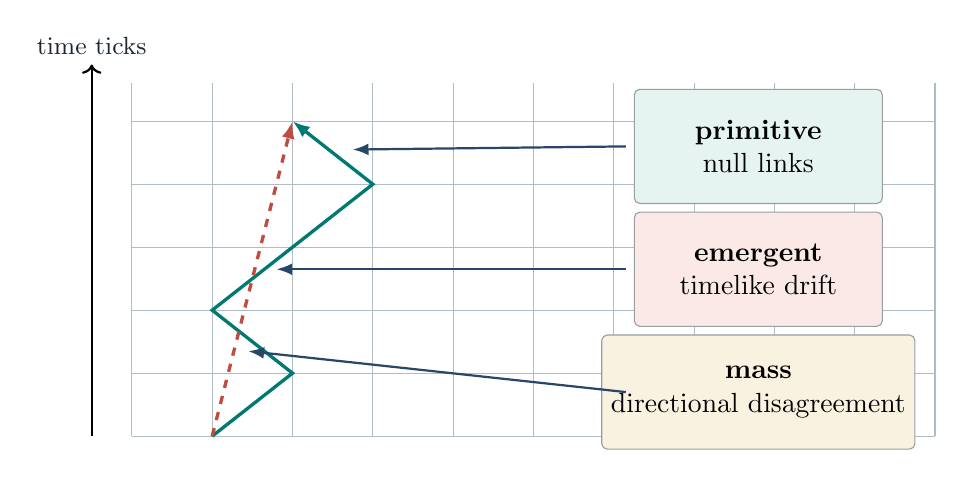
\begin{tikzpicture}[x=1.02cm,y=0.8cm]
  \foreach \x in {-5,-4,...,5} {\draw[faint] (\x,0)--(\x,5.6);}
  \foreach \y in {0,1,...,5} {\draw[faint] (-5,\y)--(5,\y);}
  \draw[->,thick] (-5.5,0)--(-5.5,5.9) node[above,label]{time ticks};
  \draw[nullray] (-4,0)--(-3,1)--(-4,2)--(-3,3)--(-2,4)--(-3,5);
  \draw[drift,dashed] (-4,0)--(-3,5);
  \node[channel,fill=paleteal] at (2.8,4.6) {\textbf{primitive}\\null links};
  \node[channel,fill=palecoral] at (2.8,2.65) {\textbf{emergent}\\timelike drift};
  \node[channel,fill=palegold] at (2.8,0.7) {\textbf{mass}\\directional disagreement};
  \draw[transport] (1.15,4.6)--(-2.25,4.55);
  \draw[transport] (1.15,2.65)--(-3.2,2.65);
  \draw[transport] (1.15,0.7)--(-3.55,1.35);
\end{tikzpicture}
\caption{Null microscopic support and timelike coarse drift are different
statements.  The dashed line is an average direction, not an additional
microscopic link.}
\label{fig:nulldrift}
\end{figure}

Four questions then organize the model:

\begin{center}
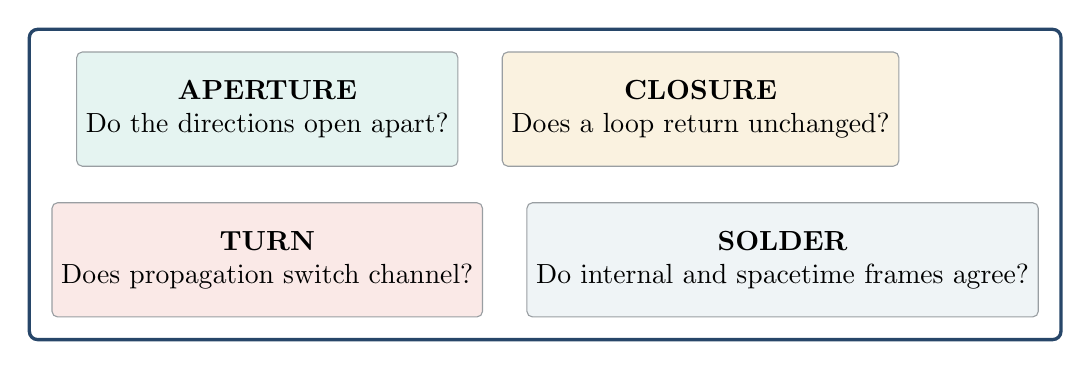
\begin{tikzpicture}[node distance=0.45cm and 0.55cm]
  \node[channel,fill=paleteal] (a) {\textbf{APERTURE}\\Do the directions open apart?};
  \node[channel,fill=palegold,right=of a] (c) {\textbf{CLOSURE}\\Does a loop return unchanged?};
  \node[channel,fill=palecoral,below=of a] (t) {\textbf{TURN}\\Does propagation switch channel?};
  \node[channel,fill=mist,right=of t] (s) {\textbf{SOLDER}\\Do internal and spacetime frames agree?};
  \node[draw=navy,very thick,rounded corners=3pt,fit=(a)(c)(t)(s),inner sep=8pt] {};
\end{tikzpicture}
\end{center}

These are not four metaphors attached after the fact.  They are the four
structural kinds of term that appear in the square of the finite
\emph{carrier} --- the single operator, studied throughout the project, that
advances the quantum amplitude by one tick.  \Clabel\quad Whether the four
kinds become kinetic, gauge, Yukawa, and gravitational terms in a continuum
theory is the central open test.

\section{Everything moves at the speed of light}
\label{sec:speed}

We mean the slogan literally --- provided you notice that ``speed'' hides
three different questions.  Distinguishing them is what lets the slogan
survive contact with physics.

\subsection*{Primitive speed}

Each allowed microscopic link lies on the light cone.  In units where
$c=1$, a step has the form
\[
  (\Delta t,\Delta\mathbf{x})=(1,\mathbf{n}),
  \qquad |\mathbf{n}|=1,
\]
so its interval is $\Delta t^2-|\Delta\mathbf{x}|^2=0$.

\subsection*{Front speed}

\Tlabel\quad For a relativistic wave equation, the fastest disturbance is
governed by the highest-derivative, or \emph{principal}, part of the equation.  If that part is
\[
  \omega^2-|\mathbf{k}|^2,
\]
the wavefront lies on the null cone.  Finite mass matrices and other
lower-order internal couplings do not change this front cone.  They do change
dispersion and interference behind the front.\footnote{For an operator whose
symbol is $q(\omega,\mathbf{k})I+L$, with $L$ independent of momentum, the
characteristic set is controlled at principal order by
$q=\omega^2-|\mathbf{k}|^2$.  The conclusion would require re-audit if a proposed
channel supplied additional derivatives of the same or higher order.}

\subsection*{Group drift}

\Tlabel\quad A massive wave packet obeys
\[
  E^2=|\mathbf{p}|^2+m^2,
  \qquad |\mathbf{v}_{\rm group}|=\frac{|\mathbf{p}|}{E}<1
  \quad(m\ne0).
\]
There is no contradiction.  The support of the microscopic propagation and
the drift of a massive packet answer different questions.

\claimbox{The strongest honest slogan.}{\Mlabel\quad All primitive propagation
in the model is null; massive motion is an emergent timelike drift produced by
coherent mixing among null channels.}

\Tlabel\quad For a Dirac fermion, each individual velocity component has
spectral values
$\pm c$.  But the three component operators do not commute, so they do not
define a simultaneous classical three-velocity of fixed magnitude $c$.  Scalar
and vector fields use different operators altogether.  The universal language
is therefore the shared null \emph{characteristic cone}, not a hidden classical
trajectory assigned to every particle and interaction channel.\footnote{For the
Dirac Hamiltonian, $\dot x_i=\alpha_i$ and each $\alpha_i$ has eigenvalues
$\pm1$, but $[\alpha_i,\alpha_j]\ne0$ for $i\ne j$.  Componentwise spectral
support therefore does not define a joint classical velocity vector.  Massive
wave-packet drift instead follows the dispersion relation and has magnitude
$|\mathbf p|/E<1$.}

\section{How mass appears when null directions disagree}

\Tlabel\quad Two future-directed null momenta can add to a timelike momentum.
Draw two lightlike arrows from the same origin (Figure~\ref{fig:aperture}).
If they point along the same ray, their
sum remains lightlike.  If they open apart, their sum moves inside the light
cone and acquires invariant mass.  This is the mirrored box of light from the
opening section, drawn as momentum arrows: each flash is massless, but the
pair is not.

\begin{figure}[ht]
\centering
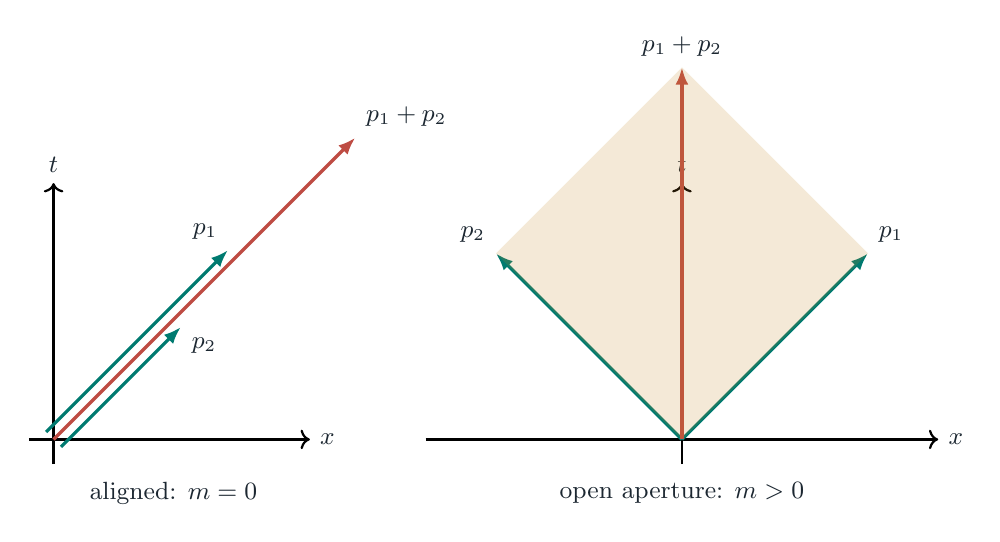
\begin{tikzpicture}[scale=1.05]
  \begin{scope}[xshift=-4.1cm]
    \draw[->,thick] (-0.3,0)--(3.1,0) node[right,label]{$x$};
    \draw[->,thick] (0,-0.3)--(0,3.1) node[above,label]{$t$};
    \draw[nullray] (-0.09,0.09)--(2.11,2.29) node[above left,label]{$p_1$};
    \draw[nullray] (0.09,-0.09)--(1.54,1.36) node[below right,label]{$p_2$};
    \draw[drift] (0,0)--(3.65,3.65) node[above right,label]{$p_1+p_2$};
    \node[label] at (1.45,-0.65) {aligned: $m=0$};
  \end{scope}
  \begin{scope}[xshift=3.5cm]
    \draw[->,thick] (-3.1,0)--(3.1,0) node[right,label]{$x$};
    \draw[->,thick] (0,-0.3)--(0,3.1) node[above,label]{$t$};
    \draw[nullray] (0,0)--(2.25,2.25) node[above right,label]{$p_1$};
    \draw[nullray] (0,0)--(-2.25,2.25) node[above left,label]{$p_2$};
    \draw[drift] (0,0)--(0,4.5) node[above,label]{$p_1+p_2$};
    \fill[gold,opacity=0.18] (0,0)--(2.25,2.25)--(0,4.5)--(-2.25,2.25)--cycle;
    \node[label] at (0,-0.65) {open aperture: $m>0$};
  \end{scope}
\end{tikzpicture}
\caption{Alignment preserves nullness.  Directional disagreement creates a
timelike sum.  The shaded area is a visual proxy for the wedge invariant.
The aligned arrows are drawn slightly offset so both remain visible; they lie
on the same ray.}
\label{fig:aperture}
\end{figure}

The finite theorem uses a $2\times2$ positive momentum matrix
\[
  P=\sum_i \psi_i\psi_i^\dagger.
\]
Each spinor $\psi_i$ supplies one rank-one, hence massless, contribution.  The
determinant is
\[
  \det P=\sum_{i<j}|\psi_i\wedge\psi_j|^2.
\]
Every term is nonnegative.  The determinant vanishes exactly when all occupied
spinors are collinear.  In the standard momentum-bispinor normalization,
$\det P=m^2$.\footnote{The identity is the $2\times2$ Cauchy--Binet formula:
$\det(\Psi\Psi^\dagger)=\sum_{i<j}|\det(\psi_i,\psi_j)|^2$.  Identifying the
determinant with Minkowski norm uses the Pauli-matrix map
$p_\mu\mapsto p_\mu\sigma^\mu$ and a fixed metric/sign convention.}

\widebox{teal}{paleteal}{\Mlabel\quad In the finite model, mass squared is
exactly the total pairwise failure of the occupied null directions to align.}

In this finite setting, mass squared is not merely \emph{modeled} by
directional disagreement; it equals it, term by term, with nothing left over.
That identity is the seed of everything that follows.\footnote{The identity is
kinematic.  Any timelike momentum can be decomposed into null momenta, so the
identity alone does not explain why a particle has one mass rather than
another; selecting a mass requires an operator, an action, a stable sector,
and ultimately a continuum limit.  Those are the later layers of the
program.}

\section{Time in steps: the checkerboard picture}
\label{sec:checkerboard}

In one spatial dimension, a null step goes either right or left.  A massive
Dirac amplitude can be represented as a sum over zigzag histories
(Figure~\ref{fig:checkerboard}).  The everyday analogue is a sailboat tacking
upwind: on every leg the boat moves at full sailing speed, yet its net
progress up the channel is slower, set by how often it comes about.  Each
corner
changes the propagation channel and contributes a factor proportional to the
mass:
\[
  A(h)=(\ii\epsilon m)^{\#\text{corners}(h)}.
\]

\begin{figure}[ht]
\centering
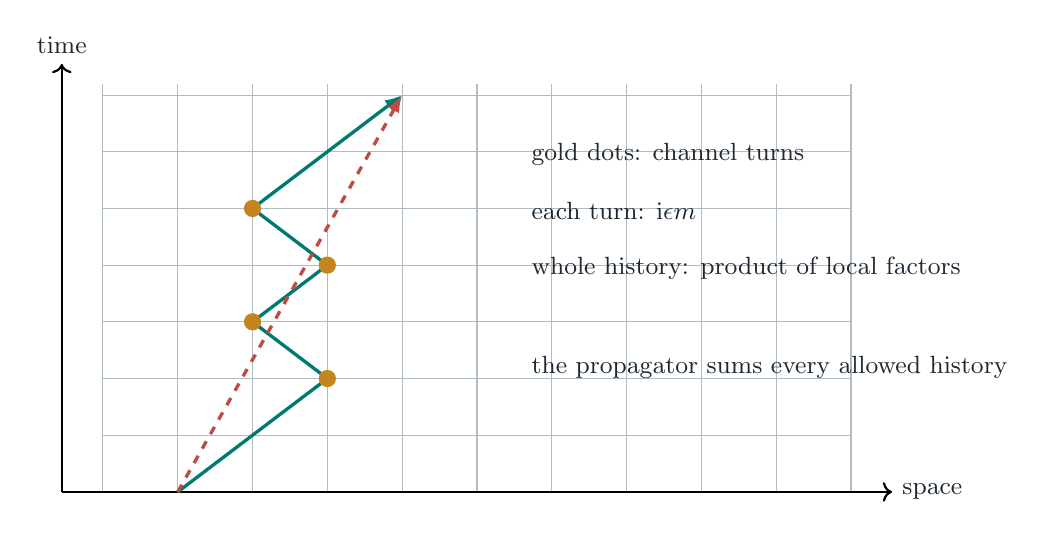
\begin{tikzpicture}[x=0.95cm,y=0.72cm]
  \foreach \x in {-5,-4,...,5} {\draw[faint] (\x,0)--(\x,7.2);}
  \foreach \y in {0,1,...,7} {\draw[faint] (-5,\y)--(5,\y);}
  \draw[->,thick] (-5.55,0)--(-5.55,7.55) node[above,label]{time};
  \draw[->,thick] (-5.55,0)--(5.55,0) node[right,label]{space};
  \coordinate (p0) at (-4,0);
  \coordinate (p1) at (-3,1);
  \coordinate (p2) at (-2,2);
  \coordinate (p3) at (-3,3);
  \coordinate (p4) at (-2,4);
  \coordinate (p5) at (-3,5);
  \coordinate (p6) at (-2,6);
  \coordinate (p7) at (-1,7);
  \draw[nullray] (p0)--(p1)--(p2)--(p3)--(p4)--(p5)--(p6)--(p7);
  \foreach \p in {p2,p3,p4,p5} {\node[circle,fill=gold,inner sep=2.2pt] at (\p) {};}
  \draw[drift,dashed] (p0)--(p7);
  \node[label,anchor=west] at (0.6,5.95) {gold dots: channel turns};
  \node[label,anchor=west] at (0.6,4.95) {each turn: $\ii\epsilon m$};
  \node[label,anchor=west] at (0.6,3.95) {whole history: product of local factors};
  \node[label,anchor=west] at (0.6,2.2) {the propagator sums every allowed history};
\end{tikzpicture}
\caption{A finite checkerboard history.  Mass enters at turns, while every
segment remains null.}
\label{fig:checkerboard}
\end{figure}

At $m=0$, every history containing a corner has zero amplitude; only straight
null histories survive.  At nonzero $m$, turned histories participate and
interfere.  \Mlabel\quad The project has checked the exact finite sum and its
discrete Dirac recursion using exact fraction arithmetic, so no rounding or
numerical approximation enters that finite statement.\footnote{Formally, the
computation runs over the Gaussian rationals: complex numbers whose real and
imaginary parts are ordinary fractions.  Every quantity in the finite
statement is represented exactly.}

The grid is a laboratory, not a portrait of space.  Everything it asserts
about physics must survive the limit in which the grid itself
disappears.\footnote{A fixed finite direction set selects a frame and cannot
by itself be exactly Lorentz invariant, and the program does not infer that
physical spacetime is literally a visible crystal.  At finite spacing the
symmetry is only the discrete symmetry of the direction set.  Recovering
Lorentz symmetry requires a scaling limit in which the propagator, not merely
a fitted dispersion curve, converges with controlled error to a
Lorentz-covariant continuum kernel.}

\subsection*{The first $3+1$ lift}

In three spatial dimensions, four directions pointing toward the vertices of a
regular tetrahedron form the smallest isotropic set of this kind.  If $c_i$
counts the number of steps in direction $i$, the finite endpoint obeys
\[
  X(c)^2=\frac{8}{3}\sum_{i<j}c_i c_j.
\]
A history using only one direction is null.  Mixing any two occupied directions
creates a positive timelike interval.

\begin{center}
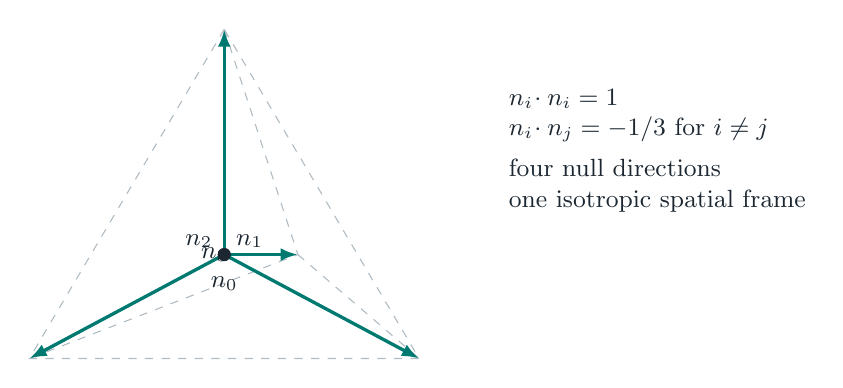
\begin{tikzpicture}[scale=1.1]
  \coordinate (o) at (0,0);
  \coordinate (a) at (0,2.6);
  \coordinate (b) at (-2.25,-1.2);
  \coordinate (c) at (2.25,-1.2);
  \coordinate (d) at (0.85,0.0);
  \draw[faint,dashed] (a)--(b)--(c)--cycle;
  \draw[faint,dashed] (a)--(d)--(b) (d)--(c);
  \foreach \p/\lab in {a/$n_0$,b/$n_1$,c/$n_2$,d/$n_3$}
    {\draw[nullray] (o)--(\p); \node[label] at ($ (\p)!1.13!(o) $) {\lab};}
  \node[dot] at (o) {};
  \node[label,align=left] at (5.0,1.2)
    {$n_i\!\cdot n_i=1$\\$n_i\!\cdot n_j=-1/3$ for $i\ne j$\\[0.4em]
     four null directions\\one isotropic spatial frame};
\end{tikzpicture}
\end{center}

\Mlabel\quad There is a sharp normalization lesson.  Equal averaging over
these four unit
directions produces $\tfrac13$ of the identity on spatial vectors.  The simplest
spin-projector recursion therefore cannot simultaneously have unit microscopic
step speed, that normalized average, and unit emergent wave speed.  This is a
constraint on one discretization, not a no-go against $3+1$ quantum
walks.\footnote{For tetrahedral unit vectors,
$\sum_{i=0}^{3}n_i n_i^T=(4/3)I_3$, so equal averaging gives $I_3/3$.  In the
minimal projector ansatz this factor rescales the spatial principal symbol.
An explicit direction register, different weights, or a more elaborate unitary
walk can change the ansatz; the finite theorem forbids only the three requested
normalizations within the simple recursion.}

\section{The four channels}

The finite carrier has schematic form
\[
  D=\sum_e c(\alpha_e)\nabla_e+\Gamma\phi.
\]
Here $c(\alpha_e)$ represents a null direction, $\nabla_e$ transports a state,
and $\Gamma\phi$ changes an internal or chiral channel.  Squaring $D$ separates
four structural effects.

\begin{center}
\begin{tabularx}{0.96\linewidth}{@{}>{\bfseries}p{0.16\linewidth}p{0.25\linewidth}X@{}}
\toprule
Channel & Visual question & Finite mathematical content\\
\midrule
\textcolor{teal}{Aperture} & Do occupied null directions open apart? &
Positive Gram/wedge terms; rank one becomes rank two; invariant mass appears.\\
\textcolor{gold!80!black}{Closure} & Does transport around a loop return unchanged? &
Commutators and holonomy; a closed path can return with a nontrivial phase or rotation.\\
\textcolor{coral}{Turn} & Does propagation switch between null channels? &
Chiral conversion and checkerboard corners; mass weights the switch.\\
\textcolor{plum}{Solder} & Do internal frames and spacetime directions agree? &
Coframe mismatch, torsion/nonmetricity-shaped terms, and a candidate geometry channel.\\
\bottomrule
\end{tabularx}
\end{center}

\subsection{Aperture: opening a timelike interior}

``Aperture'' is the opening between occupied null rays.  It is not a literal
hole in space.  Closed scissors present a single blade-line; opened scissors
enclose a wedge of area between the blades.  One ray has zero wedge area with
itself.  Two nonparallel rays
span an area, and the squared area is the mass contribution.  Aperture is the
kinematic channel and the cleanest part of the framework.

\subsection{Closure: remembering a loop}

Walk a large closed loop on the curved Earth carrying an arrow you never
deliberately rotate: start on the equator pointing north, walk to the north
pole, turn and walk back down to a different point on the equator, then walk
home along it.  The arrow comes back rotated, although you never twisted it;
the loop itself did.  Closure is the same experiment on the grid.  Place an
internal arrow at one grid point and transport it around a closed loop
(Figure~\ref{fig:closure}).
The endpoint is the starting point, but the arrow may return rotated or with a
phase.  That residual transformation is the holonomy.\footnote{For an ordered
path $e_1\cdots e_n$, the transport is the ordered product
$U_{e_n}\cdots U_{e_1}$.  Under vertex gauge transformations, open-path
transport changes by endpoint factors; for $U(1)$ a closed product is invariant,
while for a nonabelian group it is conjugated and only conjugacy-class data such
as a matrix trace is gauge invariant.}

\begin{figure}[ht]
\centering
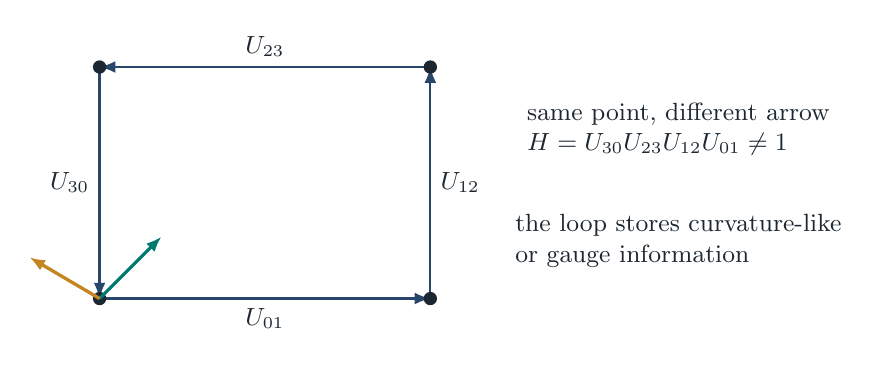
\begin{tikzpicture}[scale=1.05]
  \coordinate (a) at (-2,-1.4);
  \coordinate (b) at (2,-1.4);
  \coordinate (c) at (2,1.4);
  \coordinate (d) at (-2,1.4);
  \draw[transport] (a)--(b) node[midway,below,label]{$U_{01}$};
  \draw[transport] (b)--(c) node[midway,right,label]{$U_{12}$};
  \draw[transport] (c)--(d) node[midway,above,label]{$U_{23}$};
  \draw[transport] (d)--(a) node[midway,left,label]{$U_{30}$};
  \foreach \p in {a,b,c,d} {\node[dot] at (\p) {};}
  \draw[very thick,teal,-{Latex[length=2mm]}] (-2,-1.4)--(-1.25,-0.65);
  \draw[very thick,gold,-{Latex[length=2mm]}] (-2,-1.4)--(-2.85,-0.9);
  \node[label,align=left] at (5.0,0.65)
    {same point, different arrow\\$H=U_{30}U_{23}U_{12}U_{01}\ne1$};
  \node[label,align=left] at (5.0,-0.7)
    {the loop stores curvature-like\\or gauge information};
\end{tikzpicture}
\caption{Closure is not the geometric closing of the square; it is the failure
of transported internal data to return unchanged.}
\label{fig:closure}
\end{figure}

For complex $U(1)$ edge phases, an open path transforms only at its endpoints.
A closed-loop product is gauge invariant.  \Mlabel\quad The finite model
contains an exact
four-edge example with holonomy $\ii\ne1$ that stays $\ii$ under a nonidentity
gauge change.

\Mlabel\quad The nonabelian upgrade is now also checked.  For matrix-valued
transport, an open history transforms only at its endpoints; a closed loop is
conjugated by the gauge at its basepoint rather than left invariant; and the
loop's matrix trace survives exactly.  An explicit rational $2\times2$ example
with two noncommuting shear transports realizes all three statements: a
nonidentity gauge change visibly moves the holonomy matrix while its trace
stays fixed at $3$.  What remains open is connecting this history holonomy to
the carrier's closure block, not the holonomy algebra itself.

\subsection{Turn: converting one null channel into another}

For a massless Weyl fermion, left- and right-handed propagation decouple.  A
Dirac mass couples them.  In the checkerboard picture, the coupling is visible
as a turn; in operator language, it is the off-diagonal conversion between two
null chiral sectors.  The path picture and the matrix picture are two views of
the same local event.  In the sailboat language of
Section~\ref{sec:checkerboard}, turn is the tack: the mass sets how often the
boat comes about.

\subsection{Soldering: tying transport to spacetime}

Internal vectors do not become spacetime directions by naming them so.  A
printed map is useful only once its compass rose is aligned with north on the
actual ground, and the alignment must be rechecked from place to place.  A
\emph{coframe} is the mathematical map that performs this identification.  At
neighboring sites $x$ and $y$, let $e_x$ and $e_y$ be coframes and $U_{xy}$ the
transport between their internal frames (Figure~\ref{fig:solder}).  Their
mismatch is
\[
  T_{xy}=e_y-U_{xy}e_x.
\]

\begin{figure}[ht]
\centering
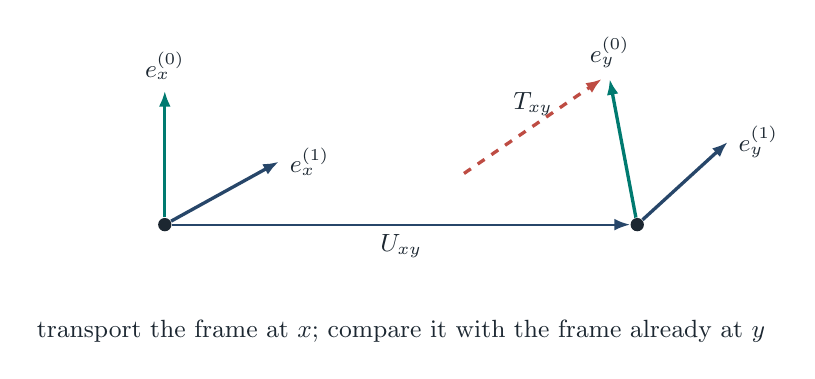
\begin{tikzpicture}[scale=1.0]
  \node[dot] (x) at (-3,0) {};
  \node[dot] (y) at (3,0) {};
  \draw[transport] (x)--(y) node[midway,below,label]{$U_{xy}$};
  \draw[very thick,teal,-{Latex[length=2mm]}] (x)--++(0,1.7) node[above,label]{$e_x^{(0)}$};
  \draw[very thick,navy,-{Latex[length=2mm]}] (x)--++(1.45,0.8) node[right,label]{$e_x^{(1)}$};
  \draw[very thick,teal,-{Latex[length=2mm]}] (y)--++(-0.35,1.85) node[above,label]{$e_y^{(0)}$};
  \draw[very thick,navy,-{Latex[length=2mm]}] (y)--++(1.15,1.05) node[right,label]{$e_y^{(1)}$};
  \draw[very thick,coral,dashed,-{Latex[length=2mm]}] (0.8,0.65)--(2.55,1.85)
    node[midway,above,label]{$T_{xy}$};
  \node[label,align=center] at (0,-1.35)
    {transport the frame at $x$; compare it with the frame already at $y$};
\end{tikzpicture}
\caption{Soldering is the comparison between an internally transported frame
and the local frame that defines spacetime directions.}
\label{fig:solder}
\end{figure}

\Mlabel\quad The finite matrix-coframe model now proves that invertible frame
changes
preserve coframe nondegeneracy, Lorentz frame changes preserve the induced
metric $e^T\eta e$, determinant-one changes preserve volume, and the quadratic
defect action $\tr(T^T\eta T)$ is frame invariant.  An exact rational boost
provides a nonzero witness.\footnote{Here a coframe is represented by an
invertible matrix $e$, the induced metric is $g=e^T\eta e$, and the edge defect
is $T_{xy}=e_y-U_{xy}e_x$.  The finite covariance theorem is algebraic.  It does
not supply differentiability, a continuum connection, or a field equation.}
This is meaningful finite geometry, but it is not
yet general relativity: there is no continuum tetrad field, Einstein equation,
or graviton in the result.

\section{Why these four belong together}

The unifying object is not the word ``mass.''  It is the square of one finite
Dirac-like carrier.  Schematically,
\[
  D^\#D
  =\underbrace{Q_A}_{\text{aperture}}
   +\underbrace{Q_C}_{\text{closure}}
   +\underbrace{Q_T}_{\text{turn}}
   +\underbrace{E}_{\text{soldering}}.
\]

The four terms are distinguished by how transport, commutators, grading, and
frame variation enter the square.  \Mlabel\quad In one explicit rational
carrier, the four
blocks are linearly independent and their coefficients can be recovered from
matrix entries.  That makes the displayed decomposition rigid for that
witness.  It does not prove that every reasonable carrier has a unique
four-channel decomposition; an abstract non-uniqueness theorem shows that an
additional physical principle is needed.

\begin{center}
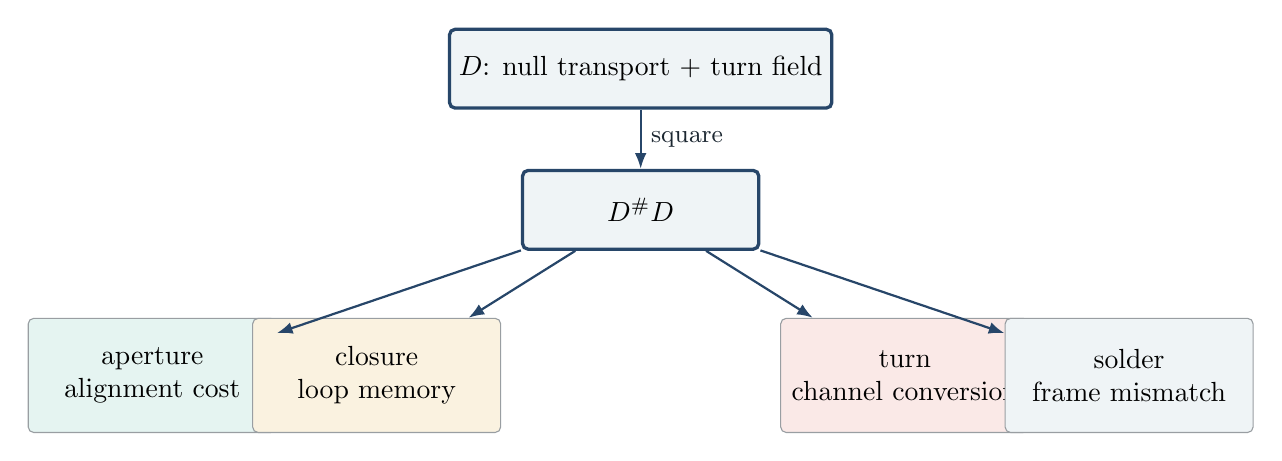
\begin{tikzpicture}[node distance=0.75cm]
  \node[draw=navy,very thick,fill=mist,rounded corners=2pt,
    minimum width=3.0cm,minimum height=1.0cm] (D) {$D$: null transport + turn field};
  \node[draw=navy,very thick,fill=mist,rounded corners=2pt,
    below=of D,minimum width=3.0cm,minimum height=1.0cm] (D2) {$D^\#D$};
  \node[channel,fill=paleteal,below left=0.85cm and 3.1cm of D2] (a) {aperture\\alignment cost};
  \node[channel,fill=palegold,below left=0.85cm and 0.25cm of D2] (c) {closure\\loop memory};
  \node[channel,fill=palecoral,below right=0.85cm and 0.25cm of D2] (t) {turn\\channel conversion};
  \node[channel,fill=mist,below right=0.85cm and 3.1cm of D2] (s) {solder\\frame mismatch};
  \draw[transport] (D)--(D2) node[midway,right,label]{square};
  \foreach \n in {a,c,t,s} {\draw[transport] (D2)--(\n);}
\end{tikzpicture}
\end{center}

This is the framework's deepest simplification: instead of proposing four
unrelated stories for mass, ask whether four familiar physical mechanisms are
the four graded faces of one operator square.  The finite algebra says that the
question is coherent.  Nature has not yet answered yes.

\section{What the picture says about particles}
\label{sec:particles}

The slogan ``all mass comes from massless primitives'' has different reach for
different species.\footnote{The broadest theorem available here is kinematic:
a future-timelike momentum can be decomposed into future-null momenta, and the
finite determinant measures their nonalignment.  A dynamical explanation of a
measured rest mass must additionally select the state and its coupling.  The
fermionic checkerboard supplies such a mass-weighted turn mechanism in a finite
model, but it does not by itself cover scalar self-mass, confinement energy, or
the observed Yukawa spectrum.}

\begin{center}
\begin{tabularx}{0.97\linewidth}{@{}>{\bfseries}p{0.17\linewidth}p{0.31\linewidth}X@{}}
\toprule
Object & Null-edge picture & Boundary\\
\midrule
Massless fermion & One Weyl propagation channel; one null momentum direction. &
Standard chiral kinematics.\\
Massive fermion & Two null chiral channels coupled by a mass term; zigzag drift. &
Finite algebra checked; literal trajectory remains interpretation.\\
Photon & Massless vector with only transverse polarizations. &
The velocity-operator story for Dirac fermions does not transfer verbatim.\\
Massive $W/Z$ & The longitudinal polarization appears together with mass; a
would-be scalar mode is reorganized into the vector field. &
Degree-of-freedom accounting is standard; the null-edge dynamics is not derived.\\
Neutrino & Dirac mass links an independent partner; Majorana mass links a state
to its charge conjugate. & Which option nature uses remains unknown.\\
Antiparticle & CPT-related orientation of the same relativistic structure. &
No explanation of the cosmic matter asymmetry follows.\\
Composite matter & Constituents and binding fields contribute to total rest
energy. & A composite object is not claimed to move microscopically at $c$.\\
Higgs scalar & No Weyl zigzag of its own. & The scalar self-mass is an explicit
exception to the universal fermionic picture.\\
\bottomrule
\end{tabularx}
\end{center}

The Higgs row matters.  The framework can describe how a scalar expectation
reorganizes fermion and vector degrees of freedom, but it does not derive the
Higgs boson's own mass from a pair of null chiral channels.  We would rather
keep a bold rule with one honest exception than trade it for a beautiful rule
that lies.

\section{Mass as lost directional simplicity}

The same $2\times2$ determinant has an information-theoretic reading.  Here
``visibility'' means what it means in the double-slit experiment: the contrast
of interference fringes, which fades as which-path --- here, which-direction
--- information becomes available.  A state
supported on one perfectly known direction is rank one and has zero determinant.
Mixing distinguishable directions raises the determinant.  In the simplest
two-direction model,
\[
  \text{mass fraction}+\text{visibility}^2=1.
\]

\begin{center}
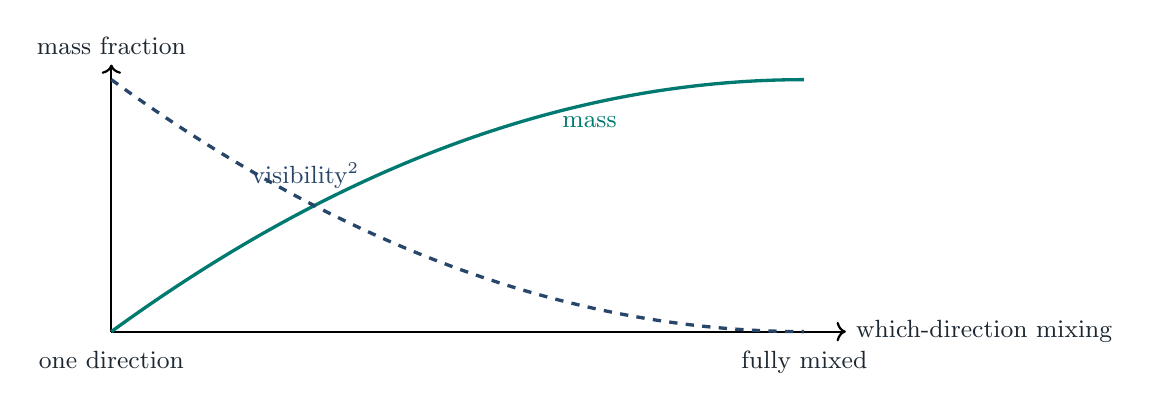
\begin{tikzpicture}[x=8.8cm,y=3.2cm]
  \draw[->,thick] (0,0)--(1.06,0) node[right,label]{which-direction mixing};
  \draw[->,thick] (0,0)--(0,1.06) node[above,label]{mass fraction};
  \draw[very thick,teal,domain=0:1,samples=80]
    plot (\x,{1-(1-\x)^2});
  \draw[very thick,navy,dashed,domain=0:1,samples=80]
    plot (\x,{(1-\x)^2});
  \node[label,teal] at (0.69,0.83) {mass};
  \node[label,navy] at (0.28,0.62) {visibility$^2$};
  \node[label,below] at (0,-0.04) {one direction};
  \node[label,below] at (1,-0.04) {fully mixed};
\end{tikzpicture}
\end{center}

This does not mean that ordinary environmental noise literally creates a
particle's rest mass.  It means that the finite invariant used as the mass
proxy is also a measure of retained directional distinguishability.  Indeed,
the model contains a signed closure operation that can lower the determinant;
closure is structured transport, not generic decoherence.

The information view is useful because it unifies several descriptions:
rank collapse for the massless boundary, continuous spectral area, linear
entropy, loss of visibility, total-variation
distinguishability, and compression cost all vanish on a single pure direction.
They are related faces of one invariant, not independent confirmations of the
physical theory.

\section{What the machine has checked}
\label{sec:machine}

\begin{center}
\fcolorbox{navy}{mist}{\begin{minipage}{0.91\linewidth}
\small
\textbf{What is Lean?}\quad Lean is a proof assistant: a computer program in
which definitions, theorems, and proofs are written in a formal language and
checked, step by logical step, by a small trusted core called the kernel.  A
statement the kernel accepts cannot hide a gap, a sign error, or an unstated
assumption, which is stronger than ``we did the algebra carefully.''  What the
kernel cannot check is whether the formal statement means what the surrounding
prose says it means.
\end{minipage}}
\end{center}

Lean verifies formal statements, not the intended interpretation.  The project
therefore treats proof and semantic audit as separate obligations.  The current
evidence ladder is:

\begin{center}
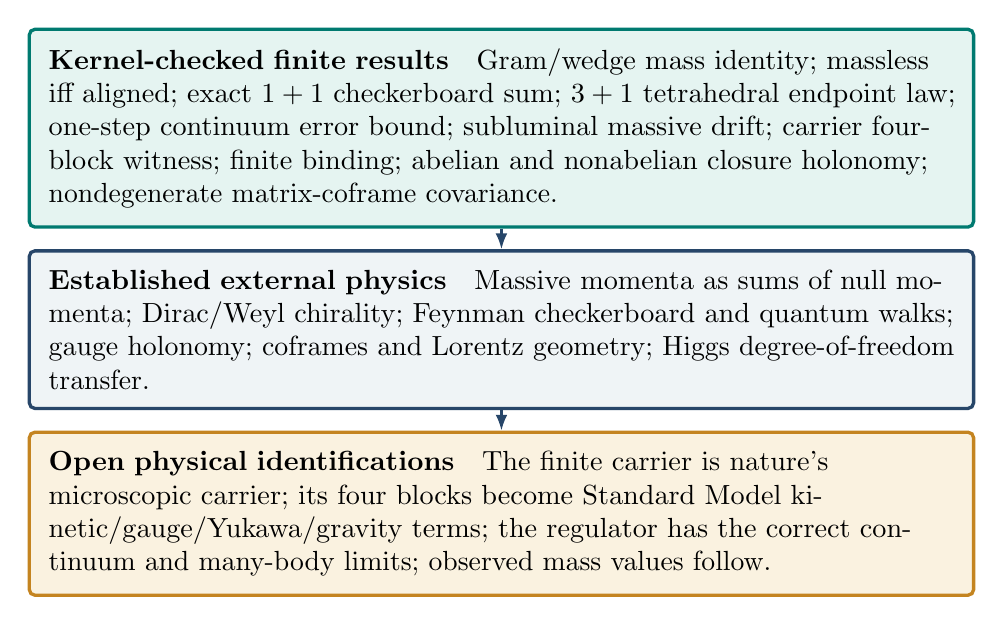
\begin{tikzpicture}[node distance=0.26cm]
  \node[draw=teal,very thick,fill=paleteal,rounded corners=2pt,
    text width=11.5cm,align=left,inner sep=7pt] (m) {
    \textbf{Kernel-checked finite results}\quad
    Gram/wedge mass identity; massless iff aligned; exact $1+1$ checkerboard
    sum; $3+1$ tetrahedral endpoint law; one-step continuum error bound;
    subluminal massive drift; carrier four-block witness; finite binding;
    abelian and nonabelian closure holonomy; nondegenerate matrix-coframe
    covariance.};
  \node[draw=navy,very thick,fill=mist,rounded corners=2pt,
    below=of m,text width=11.5cm,align=left,inner sep=7pt] (t) {
    \textbf{Established external physics}\quad
    Massive momenta as sums of null momenta; Dirac/Weyl chirality; Feynman
    checkerboard and quantum walks; gauge holonomy; coframes and Lorentz
    geometry; Higgs degree-of-freedom transfer.};
  \node[draw=gold,very thick,fill=palegold,rounded corners=2pt,
    below=of t,text width=11.5cm,align=left,inner sep=7pt] (c) {
    \textbf{Open physical identifications}\quad
    The finite carrier is nature's microscopic carrier; its four blocks become
    Standard Model kinetic/gauge/Yukawa/gravity terms; the regulator has the
    correct continuum and many-body limits; observed mass values follow.};
  \draw[transport] (m)--(t);
  \draw[transport] (t)--(c);
\end{tikzpicture}
\end{center}

Some particularly visual checked statements are worth listing plainly.

\begin{itemize}
  \item One null direction gives zero mass invariant; two nonparallel directions
        give a strictly positive rational witness.
  \item Every primitive tetrahedral step is null, while a mixed two-direction
        endpoint is timelike.
  \item The basic tetrahedral projector average has an unavoidable factor
        $1/3$; the normalization tension is a theorem, not a plotting artifact.
  \item A finite massive shell has group drift strictly below $c$, including an
        exact $3$--$4$--$5$ witness with speed squared $9/25$.
  \item A closed finite $U(1)$ loop can have nontrivial, exactly gauge-invariant
        holonomy.
  \item For noncommuting matrix transport, a closed loop's holonomy is
        conjugated by the basepoint gauge --- an explicit rational gauge change
        moves the holonomy matrix --- while its trace is exactly unchanged.
  \item A rational nonidentity Lorentz boost preserves the induced metric and a
        nonzero matrix-coframe defect action.
\end{itemize}

\section{What could prove the picture wrong}
\label{sec:kill}

A useful speculative framework should become easier to kill as it becomes more
specific.  Ours is now specific enough to shoot at; here are the seven clean
shots.

\begin{enumerate}[leftmargin=1.6em]
  \item \textbf{No continuum recovery.}  If the finite walk does not converge to
  the Dirac/Weyl propagator with controlled errors, the grid is only a toy.

  \item \textbf{Wrong characteristic cone.}  If channel terms enter at principal
  order and alter the observed null cone, the universal-speed reading fails.

  \item \textbf{Wrong field dictionary.}  If aperture, closure, turn, and
  soldering do not refine to kinetic, gauge, scalar, and geometric operators,
  the physical names must be replaced by neutral block labels.

  \item \textbf{No many-body locality.}  Single-particle quantum walks do not
  automatically produce a local quantum field theory.  Known higher-dimensional
  QCA obstructions must be confronted rather than bypassed.

  \item \textbf{No mass values.}  Structural mass identities do not predict the
  electron, quark, or neutrino spectrum.  A successful theory needs a rigid
  generation/Yukawa mechanism, not inserted constants.

  \item \textbf{No gravitational limit.}  A finite coframe defect is not yet an
  Einstein or teleparallel field equation.  Failure of the soldering channel to
  produce a legitimate continuum action would retire the gravity reading.

  \item \textbf{Scalar exception remains unexplained.}  The Higgs self-mass must
  be derived by another layer or retained openly as an input.
\end{enumerate}

\widebox{coral}{palecoral}{A theorem about a finite matrix can be completely
correct while its proposed physical interpretation is wrong.  The program is
designed so that those two verdicts can be stated independently.}

\section{The research program ahead}

The next conceptual milestones are concrete.

\begin{enumerate}[leftmargin=1.6em]
  \item Sum the now-exact ordered $3+1$ spin-projector amplitudes into a full
  endpoint kernel; bend attenuation and orientation-dependent phase are landed.
  \item Build an exactly norm-preserving tetrahedral walk with an explicit
  direction register and massive channel conversion.
  \item Prove a many-step continuum theorem rather than only a one-step error
  estimate.
  \item Instantiate the common principal-symbol theorem separately for scalar,
  Dirac, and gauge-fixed vector fields.
  \item Connect the now-checked nonabelian history holonomy to the carrier's
  closure block on each history.
  \item Relate the nondegenerate finite coframe to the actual soldering term in
  the carrier square and then to a continuum variational equation.
  \item Derive, or sharply rule out, a mechanism for three generations and
  dimensionless mass ratios.
\end{enumerate}

The goal is not to make the grid increasingly ornate.  It is to discover which
parts of the visual picture survive every change of regulator and become
continuum invariants.  Those survivors, if any, are candidates for physics.

\section{Conclusion}

The familiar statement ``massive things move slower than light'' describes the
view from far away.  In our picture it stops being true the moment you zoom
in: underneath, nothing ever slows down.  A finite null-step model makes that
claim precise:

\begin{center}
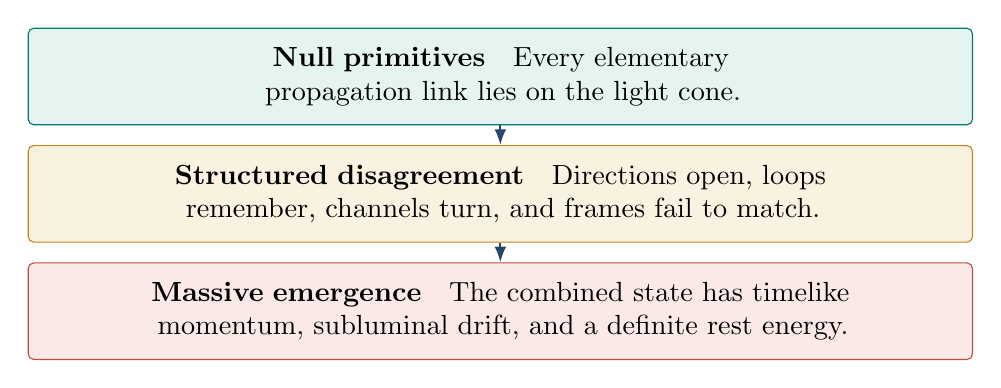
\begin{tikzpicture}[node distance=0.25cm]
  \node[draw=teal,fill=paleteal,rounded corners=2pt,text width=11.5cm,
    align=center,inner sep=7pt] (n) {\textbf{Null primitives}\quad
    Every elementary propagation link lies on the light cone.};
  \node[draw=gold,fill=palegold,rounded corners=2pt,below=of n,text width=11.5cm,
    align=center,inner sep=7pt] (d) {\textbf{Structured disagreement}\quad
    Directions open, loops remember, channels turn, and frames fail to match.};
  \node[draw=coral,fill=palecoral,rounded corners=2pt,below=of d,text width=11.5cm,
    align=center,inner sep=7pt] (m) {\textbf{Massive emergence}\quad
    The combined state has timelike momentum, subluminal drift, and a definite
    rest energy.};
  \draw[transport] (n)--(d);
  \draw[transport] (d)--(m);
\end{tikzpicture}
\end{center}

We think this is what mass \emph{is}: not a primitive substance, not a light
ray that somehow slowed down, but the invariant cost of making many lightlike
processes coexist as one stable object.\footnote{The score so far, by tier:
the aperture identity, the checkerboard sum, the subluminal drift bound, the
abelian and nonabelian closure holonomies, and the coframe covariance are
kernel-checked finite results (Section~\ref{sec:machine}); the continuum,
many-body, and mass-value layers remain open, with their kill conditions
listed in Section~\ref{sec:kill}.}  Whether nature agrees is the question the
remaining theorems and kill tests exist to answer.

\appendix
\section{Selected formal anchors}

The public-facing discussion above is grounded in the following Lean modules.
These are finite draft modules with build-enforced assumption-footprint checks;
their physical interpretation remains subject to the boundaries stated in the
text.  A technical companion manuscript (\emph{Null-Edge P1: The Origin of
Mass}, draft v3) states the same results with full definitions, conventions,
and provenance.  Module paths in the table are relative to
\texttt{PhysicsSM/Draft/NullEdge/} in the project repository
(\url{https://github.com/Pandaemonium/StandardModel}); readers with a Lean~4
toolchain can rebuild and re-verify every listed result.

\begin{center}
\small
\begin{tabularx}{0.97\linewidth}{@{}>{\ttfamily}p{0.43\linewidth}X@{}}
\toprule
Module & Payload used here\\
\midrule
GateI1/Core.lean & Gram/wedge mass identity and massless boundary\\
ExactCheckerboardPathSum.lean & Exact finite corner-weighted history sum\\
TetrahedralNullHistory.lean & $3+1$ endpoint law and $1/3$ frame factor\\
TetrahedralSpinProjectorPath.lean & Ordered bends and orientation-sensitive spin phase\\
LowerOrderChannelCausality.lean & Shared null principal cone and lower-order gate\\
DiracVelocityOperator.lean & Componentwise Dirac velocity support\\
Carrier/SubluminalBound.lean & Massive group-velocity bound\\
FourChannelRigidityCapstone.lean & Concrete four-block coefficient rigidity\\
HistoryLocalFourChannelAction.lean & Local turn action and corner phase\\
U1HistoryClosureHolonomy.lean & Gauge-invariant finite closure phase\\
NonabelianHistoryClosureHolonomy.lean & Nonabelian closure: endpoint
covariance, basepoint conjugation, gauge-invariant trace\\
NondegenerateSolderingGeometry.lean & Matrix coframe, metric, volume, and defect action\\
Carrier/DerivedInteraction.lean & Closure-derived finite binding and wrong-plane control\\
\bottomrule
\end{tabularx}
\end{center}

\section{Glossary}

\begin{description}[itemsep=0.15em,leftmargin=1.35em]
  \item[Amplitude.]  The complex number quantum mechanics attaches to each way
  an event can happen.  Amplitudes for indistinguishable alternatives add
  before being squared into probabilities, which is why histories interfere.
  \item[Null / lightlike.]  On the light cone: a step or momentum that covers
  exactly one unit of distance per unit of time (in units where $c=1$), so its
  spacetime interval is zero.
  \item[Timelike.]  Inside the light cone: slower than light.  The average
  motion of every massive object is timelike.
  \item[Invariant mass.]  The mass every observer agrees on, defined by
  $m^2=E^2-|\mathbf p|^2$.  Zero for a single flash of light; positive for a
  system of misaligned flashes.
  \item[Chirality.]  The two independent propagation channels
  (``left-handed'' and ``right-handed'') of a relativistic fermion.  Massless
  fermions keep the channels separate; a mass term couples them.
  \item[Weyl / Dirac fermion.]  A Weyl fermion is a single massless chiral
  channel; a Dirac fermion is two chiral channels coupled by a mass.
  \item[Propagator.]  The table of amplitudes for getting from one place and
  state to another in a given number of ticks.
  \item[Regulator.]  A deliberately simplified setting --- here the finite
  grid --- that makes every quantity exactly computable.  Results are trusted
  as physics only if they survive removing the regulator.
  \item[Holonomy.]  The net rotation or phase an internal arrow acquires when
  transported around a closed loop.
  \item[Coframe / soldering.]  The map that identifies internal directions
  with actual spacetime directions, and the requirement that this
  identification be consistent from place to place.
  \item[Principal part / front speed.]  The highest-derivative part of a wave
  equation, which alone controls the fastest possible wavefront.
  \item[Group velocity.]  The speed of the peak of a wave packet; the observed
  drift of a massive particle, always below $c$.
  \item[Proof assistant / kernel.]  See the box in Section~\ref{sec:machine}.
\end{description}

\section{Further reading}

The first four entries are accessible starting points for a general reader;
the rest are technical anchors for the specific mechanisms discussed above.

\begin{thebibliography}{20}

\bibitem{FeynmanQED}
R.~P.~Feynman,
\emph{QED: The Strange Theory of Light and Matter},
Princeton University Press, 1985.

\bibitem{WilczekLightness}
F.~Wilczek,
\emph{The Lightness of Being: Mass, Ether, and the Unification of Forces},
Basic Books, 2008.

\bibitem{WilczekMWM}
F.~Wilczek,
\emph{Mass without mass I: most of matter}, Physics Today 52(11) (1999) 11;
\emph{Mass without mass II: the medium is the mass-age},
Physics Today 53(1) (2000) 13.

\bibitem{Penrose}
R.~Penrose,
\emph{The Road to Reality}, Jonathan Cape, 2004.

\bibitem{FeynmanHibbs}
R.~P.~Feynman and A.~R.~Hibbs,
\emph{Quantum Mechanics and Path Integrals}, McGraw--Hill, 1965.

\bibitem{JacobsonSchulman}
T.~Jacobson and L.~S.~Schulman,
\emph{Quantum stochastics: the passage from a relativistic to a
non-relativistic path integral}, J. Phys. A 17 (1984) 375.

\bibitem{FosterJacobson}
B.~Z.~Foster and T.~Jacobson,
\emph{Spin on a 4D Feynman Checkerboard}, arXiv:1610.01142.

\bibitem{Dariano}
G.~M.~D'Ariano, N.~Mosco, P.~Perinotti, and A.~Tosini,
\emph{Path-sum solution of the Weyl Quantum Walk in 3+1 dimensions},
Phil. Trans. R. Soc. A 375 (2017) 20160394, arXiv:1705.08552.

\bibitem{Nzongani}
U.~Nzongani et al.,
\emph{Dirac quantum walk on tetrahedra}, arXiv:2404.09840.

\bibitem{ArkaniHamed}
N.~Arkani-Hamed, T.-C.~Huang, and Y.-t.~Huang,
\emph{Scattering Amplitudes For All Masses and Spins},
JHEP 11 (2021) 070, arXiv:1709.04891.

\bibitem{BaezWise}
J.~C.~Baez and D.~K.~Wise,
\emph{Teleparallel gravity as a higher gauge theory},
Commun. Math. Phys. 333 (2015) 153--186, arXiv:1204.4339.

\bibitem{MlodinowBrun}
L.~Mlodinow and T.~A.~Brun,
\emph{Quantum field theory from a quantum cellular automaton in one spatial
dimension and a no-go theorem in higher dimensions},
Phys. Rev. A 102 (2020) 042211, arXiv:2006.08927.

\end{thebibliography}

\end{document}
